% \documentclass[table]{beamer}
\documentclass[table,handout]{beamer}
\setbeameroption{show notes}
% \setbeameroption{hide notes}
% \setbeameroption{show only notes}
\usepackage{varwidth}

\newif\ifhide
\newif\ifpost
\newif\ifhideclicker

% \hidetrue
% \hideclickertrue
% \posttrue

\newcommand{\whiteout}[1]{\textcolor{white}{#1}}
% \newcommand{\whiteoutbox}[1]{\fcolorbox{white}{white}{\parbox{\dimexpr \linewidth-2\fboxsep-2\fboxrule}{\whiteout{#1}}}}
% \newcommand{\notebox}[1]{\fcolorbox{blue}{white}{\parbox{\dimexpr \linewidth-2\fboxsep-2\fboxrule}{#1}}}
\newcommand{\whiteoutbox}[1]{\fcolorbox{white}{white}{\parbox{\linewidth}{\whiteout{#1}}}}
\newcommand{\notebox}[1]{\fcolorbox{blue}{white}{\parbox{\linewidth}{#1}}}
\newcommand{\blankbox}[1]{\phantom{\varwidth{\linewidth}\whiteoutbox{#1}\endvarwidth}}
\newcommand{\blank}[1]{\phantom{\varwidth{\linewidth}#1\endvarwidth}}

\ifhide%
    \newcommand{\hmask}[1]{\blank{#1}}%
\else%
    \newcommand{\hmask}[1]{#1}%
\fi

\ifhide%
    \newcommand{\wout}[1]{\whiteout{#1}}%
\else%
    \newcommand{\wout}[1]{#1}%
\fi

\ifhide%
    \newcommand{\hignore}[1]{}%
\else%
    \newcommand{\hignore}[1]{#1}%
\fi

\ifpost%
    \newcommand{\nopost}[1]{}%
\else%
    \newcommand{\nopost}[1]{#1}%
\fi

\ifhideclicker%
    \newcommand{\clickerslide}[1]{\stepcounter{clickerQuestionCounter}%
        \begin{frame}[t]
            \textcolor{blue}{Q \arabic{clickerQuestionCounter}:}
        \end{frame}}
\else%
    \newcommand{\clickerslide}[1]{#1}%
\fi

\ifhide%
    \newcommand{\hidebox}[1]{\blank{#1}}%
\else%
    \newcommand{\hidebox}[1]{\notebox{#1}}%
\fi

\ifhide%
    \newcommand{\wbox}[1]{\whiteoutbox{#1}}%
\else%
    \newcommand{\wbox}[1]{\notebox{#1}}%
\fi

\ifhide%
    \newcommand{\nbox}[1]{\blankbox{#1}}%
\else%
    \newcommand{\nbox}[1]{\notebox{#1}}%
\fi

\ifhideclicker%
    \newcommand{\clickeranswer}[1]{#1}%
\else%
    \ifhide%
        \newcommand{\clickeranswer}[1]{#1}%
    \else%
        \newcommand{\clickeranswer}[1]{\textbf{\textcolor{blue}{#1}}}%
    \fi
\fi

\usepackage{beamerthemesplit}
% \usetheme{boxes}
\usetheme{Malmoe}
\usecolortheme{seahorse}
% \usecolortheme{seagull}
\usepackage{ifthen}
\usepackage{xspace}
\usepackage{multirow}
\usepackage{multicol}
\usepackage{booktabs}
\usepackage{xcolor}
\usepackage{wasysym}
\usepackage{comment}
\usepackage{hyperref}
\hypersetup{pdfborder={0 0 0}, colorlinks=true, urlcolor=blue, linkcolor=blue, citecolor=blue}
\usepackage{changepage}
\usepackage[compatibility=false]{caption}
\captionsetup[figure]{font=scriptsize, labelformat=empty, textformat=simple, justification=centering, skip=2pt}
\usepackage{tikz}
\usetikzlibrary{trees,calc,backgrounds}

\usepackage[bibstyle=joaks-slides,maxcitenames=3,mincitenames=1,backend=biber]{biblatex}

\newrobustcmd*{\shortfullcite}{\AtNextCite{\renewbibmacro{title}{}\renewbibmacro{in:}{}\renewbibmacro{number}{}}\fullcite}

\newrobustcmd*{\footlessfullcite}{\AtNextCite{\renewbibmacro{title}{}\renewbibmacro{in:}{}}\footfullcite}

% Make all footnotes smaller
% \renewcommand{\footnotesize}{\scriptsize}

\definecolor{myGray}{gray}{0.9}
\colorlet{rowred}{red!30!white}

\setbeamertemplate{blocks}[rounded][shadow=true]

\setbeamercolor{defaultcolor}{bg=structure!30!normal text.bg,fg=black}
\setbeamercolor{block body}{bg=structure!30!normal text.bg,fg=black}
\setbeamercolor{block title}{bg=structure!50!normal text.bg,fg=black}

\newenvironment<>{varblock}[2][\textwidth]{%
  \setlength{\textwidth}{#1}
  \begin{actionenv}#3%
    \def\insertblocktitle{#2}%
    \par%
    \usebeamertemplate{block begin}}
  {\par%
    \usebeamertemplate{block end}%
  \end{actionenv}}

\newenvironment{displaybox}[1][\textwidth]
{
    \centerline\bgroup\hfill
    \begin{beamerboxesrounded}[lower=defaultcolor,shadow=true,width=#1]{}
}
{
    \end{beamerboxesrounded}\hfill\egroup
}

\newenvironment{onlinebox}[1][4cm]
{
    \newbox\mybox
    \newdimen\myboxht
    \setbox\mybox\hbox\bgroup%
        \begin{beamerboxesrounded}[lower=defaultcolor,shadow=true,width=#1]{}
    \centering
}
{
    \end{beamerboxesrounded}\egroup
    \myboxht\ht\mybox
    \raisebox{-0.25\myboxht}{\usebox\mybox}\hspace{2pt}
}

\newenvironment{mydescription}{
    \begin{description}
        \setlength{\leftskip}{-1.5cm}}
    {\end{description}}

\newenvironment{myitemize}{
    \begin{itemize}
        \setlength{\leftskip}{-.3cm}}
    {\end{itemize}}

% footnote without a marker
\newcommand\barefootnote[1]{%
  \begingroup
  \renewcommand\thefootnote{}\footnote{#1}%
  \addtocounter{footnote}{-1}%
  \endgroup
}

% define formatting for footer
\newcommand{\myfootline}{%
    {\it
    \insertshorttitle
    \hspace*{\fill} 
    \insertshortauthor, \insertshortinstitute
    % \ifx\insertsubtitle\@empty\else, \insertshortsubtitle\fi
    \hspace*{\fill}
    \insertframenumber/\inserttotalframenumber}}

% set up footer
\setbeamertemplate{footline}{%
    \usebeamerfont{structure}
    \begin{beamercolorbox}[wd=\paperwidth,ht=2.25ex,dp=1ex]{frametitle}%
        % \Tiny\hspace*{4mm}\myfootline\hspace{4mm}
        \tiny\hspace*{4mm}\myfootline\hspace{4mm}
    \end{beamercolorbox}}

% remove navigation bar
\beamertemplatenavigationsymbolsempty

\makeatletter
    \newenvironment{noheadline}{
        \setbeamertemplate{headline}[default]
        \def\beamer@entrycode{\vspace*{-\headheight}}
    }{}
\makeatother

\newcounter{clickerQuestionCounter}
\ifhideclicker%
\newenvironment{clickerquestion}
{ \stepcounter{clickerQuestionCounter}
  \begin{enumerate}[Q \arabic{clickerQuestionCounter}:]\color{white} }
{ \end{enumerate} }
\else%
\newenvironment{clickerquestion}
{ \stepcounter{clickerQuestionCounter}
  \begin{enumerate}[Q \arabic{clickerQuestionCounter}:] }
{ \end{enumerate} }
\fi

\ifhideclicker%
\newenvironment{clickeroptions}
{ \begin{enumerate}[\begingroup\color{white} 1)\endgroup]\color{white} }
{ \end{enumerate} }
\else%
\newenvironment{clickeroptions}
{ \begin{enumerate}[\begingroup\color{red} 1)\endgroup] }
{ \end{enumerate} }
\fi


\tikzstyle{centered} = [align=center, text centered, font=\sffamily\bfseries]
\tikzstyle{skip} = [centered, inner sep=0pt, fill]
\tikzstyle{empty} = [centered, inner sep=0pt]
\tikzstyle{inode} = [centered, circle, minimum width=4pt, fill=black, inner sep=0pt]
\tikzstyle{tnode} = [centered, circle, inner sep=1pt]
\tikzset{
  % edge styles
  level distance=10mm,
  mate/.style={edge from parent/.style={draw,distance=3pt}},
  mleft/.style={grow=left, level distance=10mm, edge from parent path={(\tikzparentnode.west)--(\tikzchildnode.east)}},
  mright/.style={grow=right, level distance=10mm, edge from parent path={(\tikzparentnode.east)--(\tikzchildnode.west)}},
  % node styles
  male/.style={rectangle,minimum size=4mm,fill=gray!80},
  female/.style={circle,minimum size=4mm,fill=gray!80},
  amale/.style={male,fill=red},
  afemale/.style={female,fill=red},
}

\newcommand{\highlight}[1]{\textcolor{violet}{\textit{\textbf{#1}}}}
\newcommand{\super}[1]{\ensuremath{^{\textrm{\sffamily #1}}}}
\newcommand{\sub}[1]{\ensuremath{_{\textrm{\sffamily #1}}}}
\newcommand{\dC}{\ensuremath{^\circ{\textrm{C}}}}
\newcommand{\tb}{\hspace{2em}}
\providecommand{\e}[1]{\ensuremath{\times 10^{#1}}}
\newcommand{\myHangIndent}{\hangindent=5mm}

\newcommand{\spp}[1]{\textit{#1}}

\newcommand\mybullet{\leavevmode%
\usebeamertemplate{itemize item}\hspace{.5em}}

\makeatletter
\newcommand*{\rom}[1]{\expandafter\@slowromancap\romannumeral #1@}
\makeatother

\newcommand{\blankslide}{{\setbeamercolor{background canvas}{bg=black}
\setbeamercolor{whitetext}{fg=white}
\begin{frame}<handout:0>[plain]
\end{frame}}}

\newcommand{\whiteslide}{
\begin{frame}<handout:0>[plain]
\end{frame}}

\newcommand{\f}[1]{\ensuremath{F_{#1}}}
\newcommand{\x}[1]{X\ensuremath{^{#1}}}
\newcommand{\y}[1]{Y\ensuremath{^{#1}}}

% Population growth macros
\newcommand{\popsize}[1]{\ensuremath{N_{#1}}}
\newcommand{\popgrowthratediscrete}[1]{\ensuremath{\lambda_{#1}}}
\newcommand{\popgrowthrate}[1]{\ensuremath{r_{#1}}}
\newcommand{\ptime}{\ensuremath{t}\xspace}

\tikzset{hide on/.code={\only<#1>{\color{white}}}}
\tikzset{
    invisible/.style={opacity=0},
    visible on/.style={alt={#1{}{invisible}}},
    alt/.code args={<#1>#2#3}{%
        \alt<#1>{\pgfkeysalso{#2}}{\pgfkeysalso{#3}}
        % \pgfkeysalso doesn't change the path
    },
}

\bibliography{../bib/references}
\author[J.\ Oaks]{
    %Jamie R.\ Oaks\inst{1}
    Jamie R.\ Oaks
}
\institute[BIOL 180]{
    \inst{}%
        BIOL 180: Introductory Biology
}



\title[Dihybrid Crosses; Mitosis \& Meiosis]{Dihybrid Crosses; Mitosis \& Meiosis}
% \date{\today}
\date{April 7, 2015}

\begin{document}

\begin{noheadline}
\maketitle
\end{noheadline}

\nopost{
\begin{noheadline}
\begin{frame}[c]
    \vspace{-6mm}
    \begin{center} 
        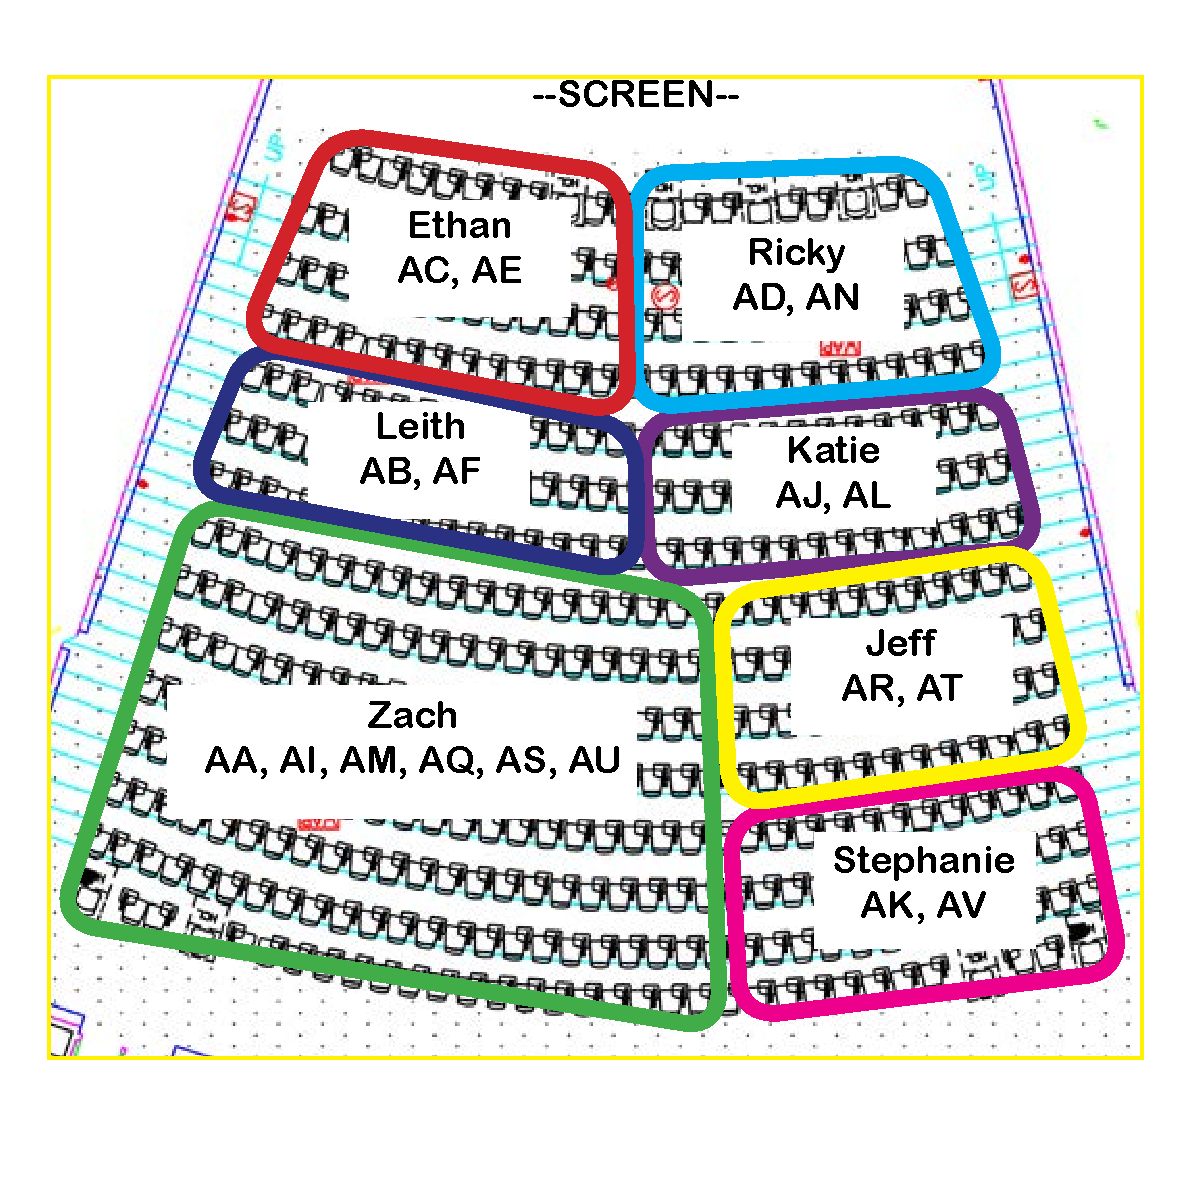
\includegraphics[height=1.3\textheight]{../images/seating-chart.pdf}
    \end{center}
\end{frame}
\end{noheadline}
}


\begin{noheadline}
\begin{frame}
\frametitle{Today's issues:}
% \tableofcontents[subsectionstyle=hide]
\begin{enumerate}
    \item How are alleles from different genes transmitted to offspring
        (together, or independently of each other?
    \item What is the physical basis of Mendel's rules?
        \begin{enumerate}
            \item Mitosis: How cells divide during asexual reproduction and
                during growth
            \item Meiosis: How cells divide prior to formation of eggs and
                sperm (sexual reproduction)
        \end{enumerate}
\end{enumerate}
\end{frame}
\end{noheadline}

\section{Transmission of alleles from different genes}

\clickerslide{
\begin{noheadline}
\begin{frame}[t]
    \frametitle{Interpreting a dihybrid cross}
    \vspace{-5mm}
    \begin{clickerquestion}
        \item Predict results of this cross, \uppercase{assuming the alleles of
                different genes do \highlight{not} stay together}
    \end{clickerquestion}

    \vspace{-2mm}
    \begin{center}
        $PPTT \,\textrm{\male} \times pptt \,\textrm{\female}$
    \end{center}
    \vspace{-3mm}
    Gamete genotypes: \hmask{\highlight{All $PT$ for male, and all $pt$ for female}} \\
    \f{1} genotypes: \hmask{\highlight{All $PpTt$}} \\
    % What happens when an \f{1} offspring self-fertilizes? \\
    % \f{1} parental genotypes: \hmask{\highlight{$PT//pt \times PT//pt$}} \\
    \f{1} gamete genotypes: \hmask{\highlight{$\frac{1}{4}PT: \frac{1}{4}Pt : \frac{1}{4}pT : \frac{1}{4}pt$}} \\
    Punnett square (\f{1} $\times$ \f{1}):

    \vspace{-2mm}
    \begin{table}%[htbp]
        \centering
        \begin{tabular}{ l | l l l l}
            & \hmask{\highlight{$PT$}} & \hmask{\highlight{$Pt$}} & \hmask{\highlight{$pT$}} & \hmask{\highlight{$pt$}} \\
            \hline
            \hmask{\highlight{$PT$}} & \hmask{\highlight{$PPTT$}} & \hmask{\highlight{$PPTt$}} & \hmask{\highlight{$PpTT$}} & \hmask{\highlight{$PpTt$}} \\
            \hmask{\highlight{$Pt$}} & \hmask{\highlight{$PPTt$}} & \hmask{\highlight{$PPtt$}} & \hmask{\highlight{$PpTt$}} & \hmask{\highlight{$Pptt$}} \\
            \hmask{\highlight{$pT$}} & \hmask{\highlight{$PpTT$}} & \hmask{\highlight{$PpTt$}} & \hmask{\highlight{$ppTT$}} & \hmask{\highlight{$ppTt$}} \\
            \hmask{\highlight{$pt$}} & \hmask{\highlight{$PpTt$}} & \hmask{\highlight{$Pptt$}} & \hmask{\highlight{$ppTt$}} & \hmask{\highlight{$pptt$}} \\
        \end{tabular}
    \end{table}
    \vspace{-2mm}

    Ratio of \f{2} phenotypes:
    \begin{clickeroptions}
        \item 3 purple/tall: 1 white/dwarf
        \item 1 purple/tall: 1 white/dwarf
        \item 9 purple/tall: 1 purple/dwarf: 1 white/tall: 1 white/dwarf
        \item \clickeranswer{9 purple/tall: 3 purple/dwarf: 3 white/tall: 1 white/dwarf}
    \end{clickeroptions}
\end{frame}
\end{noheadline}
}

\begin{frame}[t]
    \frametitle{Mendel's actual results}
    \vspace{-6mm}
    \begin{center}
        $YYRR  \times yyrr$
    \end{center}
    \vspace{-4mm}
    \begin{table}%[htbp]
        \centering
        \begin{tabular}{l l}
            $Y$ = yellow & $R$ = round \\
            $y$ = green & $r$ = wrinkled \\
        \end{tabular}
    \end{table}

    \vspace{-2mm}
    \uncover<2->{
    All \f{1}s had yellow and round seeds ($YyRr$) \\
    }

    \vspace{2mm}
    \uncover<3->{
    When \f{1}s self-fertilized, phenotypes of \f{2} offspring were:
    \vspace{-3mm}
    \begin{table}%[htbp]
        \centering
        \begin{tabular}{l l}
            yellow-round & 315 \\
            green-round & 108 \\
            yellow-wrinkled & 101 \\
            green-wrinkled & 32 \\
            TOTAL & 556 \\
        \end{tabular}
    \end{table}
    }

    \vspace{-3mm}
    \uncover<4->{
    \begin{clickerquestion}
        \item What are the \textbf{\textit{frequencies}} of the observed phenotypes?
            What hypothesis does this experiment support?
        \begin{clickeroptions}
            \item 9 y-r: 3 g-r: 3 y-w: 1 g-w; independent assortment
            \item 9 y-r: 3 g-r: 3 y-w: 1 g-w; dependent assortment
            \item \clickeranswer{0.57 y-r, 0.19 g-r, 0.18 y-w, 0.06 g-w; independent assortment}
            \item 0.57 y-r, 0.19 g-r, 0.18 y-w, 0.06 g-w; dependent assortment
        \end{clickeroptions}
    \end{clickerquestion}
    }
\end{frame}

\begin{frame}
    \frametitle{Mendel's actual results}
    \begin{itemize}[<+->]
        \item \highlight{Note:} Other combinations of two traits behaved the
            same way.
        \item Mendel's conclusion: The segregation of alleles of different
            genes occurs independently of each other.
            \begin{itemize}
                \item \textbf{This is the principle of independent assortment}
            \end{itemize}
        \item \highlight{Note:} The principle of independent assortment is
            misleading.
    \end{itemize}

    \note[item]{Do the ``sometimes principle'' and Cookie Monster}
\end{frame}


\section{The physical basis of Mendel's rules}

\begin{frame}
    \begin{itemize}
        \item To understand the physical basis of Mendel's rules and how
            genetic variation is generated in populations, we need to examine
            two types of cell division that were first described in the late
            1800s---mitosis and meiosis. 

            \vspace{5mm}
        \item But first!
            \begin{itemize}
                \item What are chromosomes (``colored bodies'')?
            \end{itemize}
    \end{itemize}
\end{frame}

\subsection{Chromosomes}

\begin{frame}
    \begin{itemize}
        \item Chromosomes come in different types, distinguished by size and
            shape (morphology). Draw 5:
        \vspace{4cm}
        \item In many organisms, there are 2 of each type of chromosome
            present. Draw the second of each type (above).
        \item Pairs of each type are said to be homologous (they are homologs).
            Circle the 5 pairs of homologs.
    \end{itemize}

    \note[item]{Draw 5 different types of ``lines''}
    \note[item]{Add a matching to each of the 5, making total of 10}
    \note[item]{Circle the ``identical pairs''}
    \note[item]{\textbf{Ask:} Ploidy? Haploid or diploid?}
    \note[item]{\textbf{Ask:} Haploid number?}
\end{frame}

\begin{frame}
    \frametitle{Key notation:}
    \begin{itemize}
        \item Use $n$ to indicate the \highlight{number of different types} of
            chromosomes found in a species
        \item Use a numeral before the $n$ to indicate \highlight{the number of
                each type} present
        \item Which is the ploidy?
            \nbox{\highlight{the number of each type}; the number before $n$;
                e.g., $\highlight{2}n=46$}
        \item Which is the haploid number?
            \nbox{\highlight{the number of different types ($n$)}; e.g.,
                $2\highlight{n}=46$, $\highlight{n=23}$}
        \item What's the difference between a homolog and a chromatid?
            \nbox{Homologs are separate chromosomes (from different parents;
                \highlight{different genetic info}).  Sister chromatids are
                identical copies of the same chromosome; physically connected}
    \end{itemize}
\end{frame}

\clickerslide{
\begin{frame}[t]
    \vspace{-3mm}
    \begin{clickerquestion}
        \item What is the haploid number and ploidy of this cell?
    \end{clickerquestion}
    \vspace{-1mm}
    \begin{center} 
        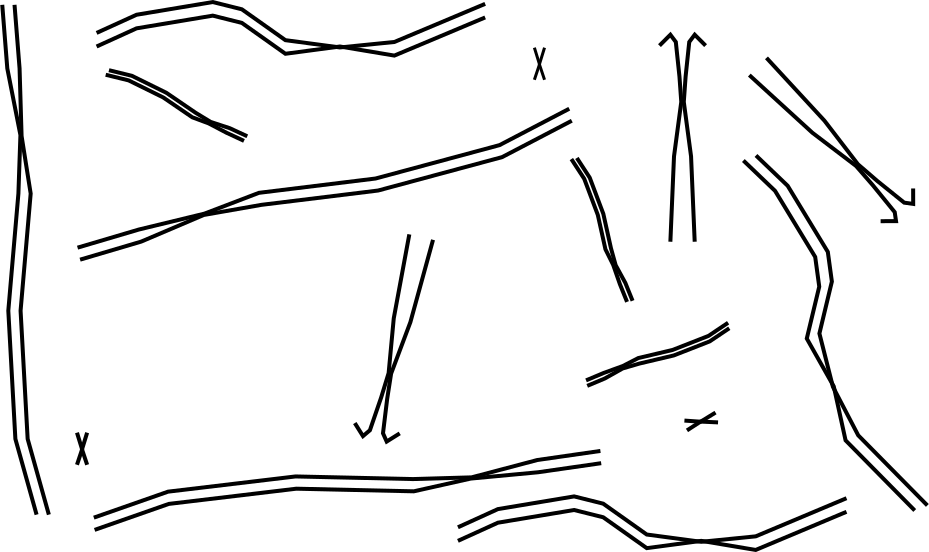
\includegraphics[width=0.7\textwidth]{../images/chromosomes.pdf}
    \end{center}
    \vspace{-3mm}
    \begin{table}%[htbp]
        \centering
        \begin{tabular}{ l c l }
            & Haploid \# & Ploidy \\
            \hline
            \textcolor{red}{1)} & \clickeranswer{5} & \clickeranswer{3 (triploid)} \\ 
            \textcolor{red}{2)} & 15 & 1 (haploid) \\ 
            \textcolor{red}{3)} & 15 & 2 (diploid) \\ 
            \textcolor{red}{4)} & 15 & 3 (triploid) \\ 
            \textcolor{red}{5)} & 30 & 1 (haploid) \\ 
        \end{tabular}
    \end{table}
\end{frame}
}

\begin{frame}[b]
    \begin{center} 
        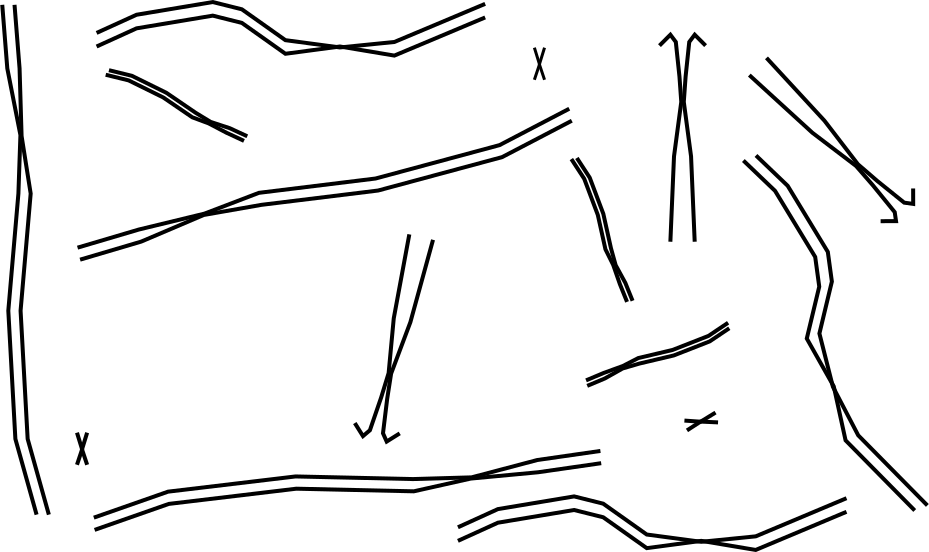
\includegraphics[width=0.65\textwidth]{../images/chromosomes.pdf}
    \end{center}
    \vspace{-3mm}
\end{frame}

\begin{frame}[t]
    \begin{adjustwidth}{-2em}{-2em}
    \begin{table}%[htbp]
        \centering
        \begin{tabular}{ p{0.45\linewidth} p{0.45\linewidth} }
            Draw a haploid set of unreplicated chromosomes in a species where
            $n=6$: &
            \hmask{\highlight{\small Draw 6 ``threads'', each a distinct
                    size/shape}} \\[3ex]
            Draw the unreplicated chromosomes of a diploid cell in a species
            where $n=5$ and $2n=10$: &
            \hmask{\highlight{\small Draw 5 ``threads'', each with a distinct
                    size/shape, then draw a second ``thread'' of each type for
                    a total of 10}} \\[3ex]
            Draw the replicated chromosomes of a diploid cell in a species
            where $n=3$ and $2n=6$: &
            \hmask{\highlight{\small Draw 3 ``double-threads'', each with a
                    distinctive size/shape, then draw a second of each type for
                    a total of 6 ``double-threads''}} \\
        \end{tabular}
    \end{table}
    \end{adjustwidth}
\end{frame}

\clickerslide{
\begin{frame}
    \begin{clickerquestion}
        \item Prior to replication of the chromosomes, a cell has $2n=6$
            chromosomes. What is the ploidy and haploid number of the cell
            after the chromosomes replicate?
    \end{clickerquestion}
    \begin{table}%[htbp]
        \centering
        \begin{tabular}{ l c l }
            & Haploid \# & Ploidy \\
            \hline
            \textcolor{red}{1)} & \clickeranswer{3} & \clickeranswer{2 (diploid)} \\ 
            \textcolor{red}{2)} & 6 & 2 (diploid) \\ 
            \textcolor{red}{3)} & 12 & 2 (diploid) \\ 
            \textcolor{red}{4)} & 12 & 1 (haploid) \\ 
            \textcolor{red}{5)} & 3 & 4 (tetraploid) \\ 
        \end{tabular}
    \end{table}
    \nbox{The cell is still diploid; the only difference is that the
        chromosomes are now comprised of sister chromatids}
\end{frame}
}


\subsection{Mitosis}

\begin{frame}[t]
    \frametitle{An overview of mitosis}
        \vspace{-3mm}
        \highlight{Mitosis:} The process responsible for asexual reproduction and
            growth in multicellular organisms. 
    \begin{adjustwidth}{-3em}{-3em}

    \vspace{1mm}
    \begin{table}%[htbp]
        \centering
        \begin{tabular}{ p{0.45\linewidth} p{0.45\linewidth} }
            Draw $2n=4$ (unreplicated) & \\[5ex]
            Chromosomes replicate & \\[5ex]
            Chromosomes line up & \\[5ex]
            Sister chromatids separate & \\[5ex]
            Cell divides & \\
        \end{tabular}
    \end{table}
    \end{adjustwidth}
    What is the ploidy of the daughter cells? \hmask{\highlight{Diploid!}}
    \note[item]{Note: cytokinesis is independent of mitosis---ask what happens
        if you get mitosis without cytokinesis}
\end{frame}


\subsection{Meiosis}

\begin{frame}
    \highlight{Meiosis:} The process responsible for sexual reproduction in
    multicellular organisms.

    \vspace{4mm}
    \begin{itemize}
        \item How does it happen?

        \vspace{4mm}
        \item \highlight{NOTE:} Meiosis consists of two divisions
    \end{itemize}
\end{frame}

\begin{noheadline}
\begin{frame}[t]
    \frametitle{An overview of meiosis I}
    \begin{adjustwidth}{-3em}{-3em}

        \vspace{-3mm}
    \begin{table}%[htbp]
        \centering
        \begin{tabular}{ p{0.45\linewidth} p{0.45\linewidth} }
            Draw $2n=4$ (unreplicated) & \\[5ex]
            Chromosomes replicate & \\[5ex]
            {\small Homologs synapse; crossing over occurs} & \\[5ex]
            Homologs line up & \\[5ex]
            Homologs pull apart & \\[5ex]
            Cell divides & \\
        \end{tabular}
    \end{table}
    \end{adjustwidth}
    \vspace{3mm}
    What is the ploidy of the daughter cells? \hmask{\highlight{Haploid!}}
\end{frame}
\end{noheadline}

\begin{noheadline}
\begin{frame}[t]
    \frametitle{An overview of meiosis II (same in both daughter cells)}
    \begin{adjustwidth}{-3em}{-3em}

        \vspace{-1mm}
    \begin{table}%[htbp]
        \centering
        \begin{tabular}{ p{0.45\linewidth} p{0.45\linewidth} }
            Chromosomes line up & \\[12ex]
            Sister chromatids pull apart & \\[12ex]
            Cell divides & \\
        \end{tabular}
    \end{table}
    \end{adjustwidth}
    \vspace{1.5cm}
    What is the ploidy of the daughter cells? \hmask{\highlight{Haploid!}}
\end{frame}
\end{noheadline}

\begin{noheadline}
\begin{frame}[t]
    \frametitle{What are the consequences of mitosis and meiosis?}
        \vspace{-4mm}
        Fill out table based on our examples of diploid cells:
    \begin{adjustwidth}{-3em}{-3em}

        \vspace{3mm}
    \begin{table}%[htbp]
        \centering
        \begin{tabular}{ p{0.12\linewidth} | p{0.38\linewidth} | p{0.38\linewidth} }
            & Mitosis & Meiosis \\
            \hline
            Start & \hmask{\highlight{Diploid cell with replicated chromosomes}} & 
                    \hmask{\highlight{Diploid cell with replicated chromosomes}} \\[3ex]
            \hline
            End & \hmask{\highlight{2 diploid cells with unreplicated chromosomes}} & 
                    \hmask{\highlight{4 haploid cells with unreplicated chromosomes}} \\[3ex]
            \hline
            {\scriptsize Chromosomes same or different as parent cell?} & \hmask{\highlight{Same}} & \hmask{\highlight{Different}} \\
        \end{tabular}
    \end{table}
    \end{adjustwidth}
\end{frame}
\end{noheadline}

\end{document}

\begin{noheadline}
\begin{frame}
    \begin{clickerquestion}
        \item 
        \begin{clickeroptions}
            \item 
            \item 
            \item 
            \item 
        \end{clickeroptions}
    \end{clickerquestion}
\end{frame}
\end{noheadline}
